\section{Ausblick}

\subsection{Funktionsmuster}
\begin{frame}
	\frametitle{Funktionsmuster\hfill{}\footnotesize \group}
	\framesubtitle{Ballnachführung}
	\begin{columns}
		\begin{column}{0.5\textwidth}
			\begin{figure}
				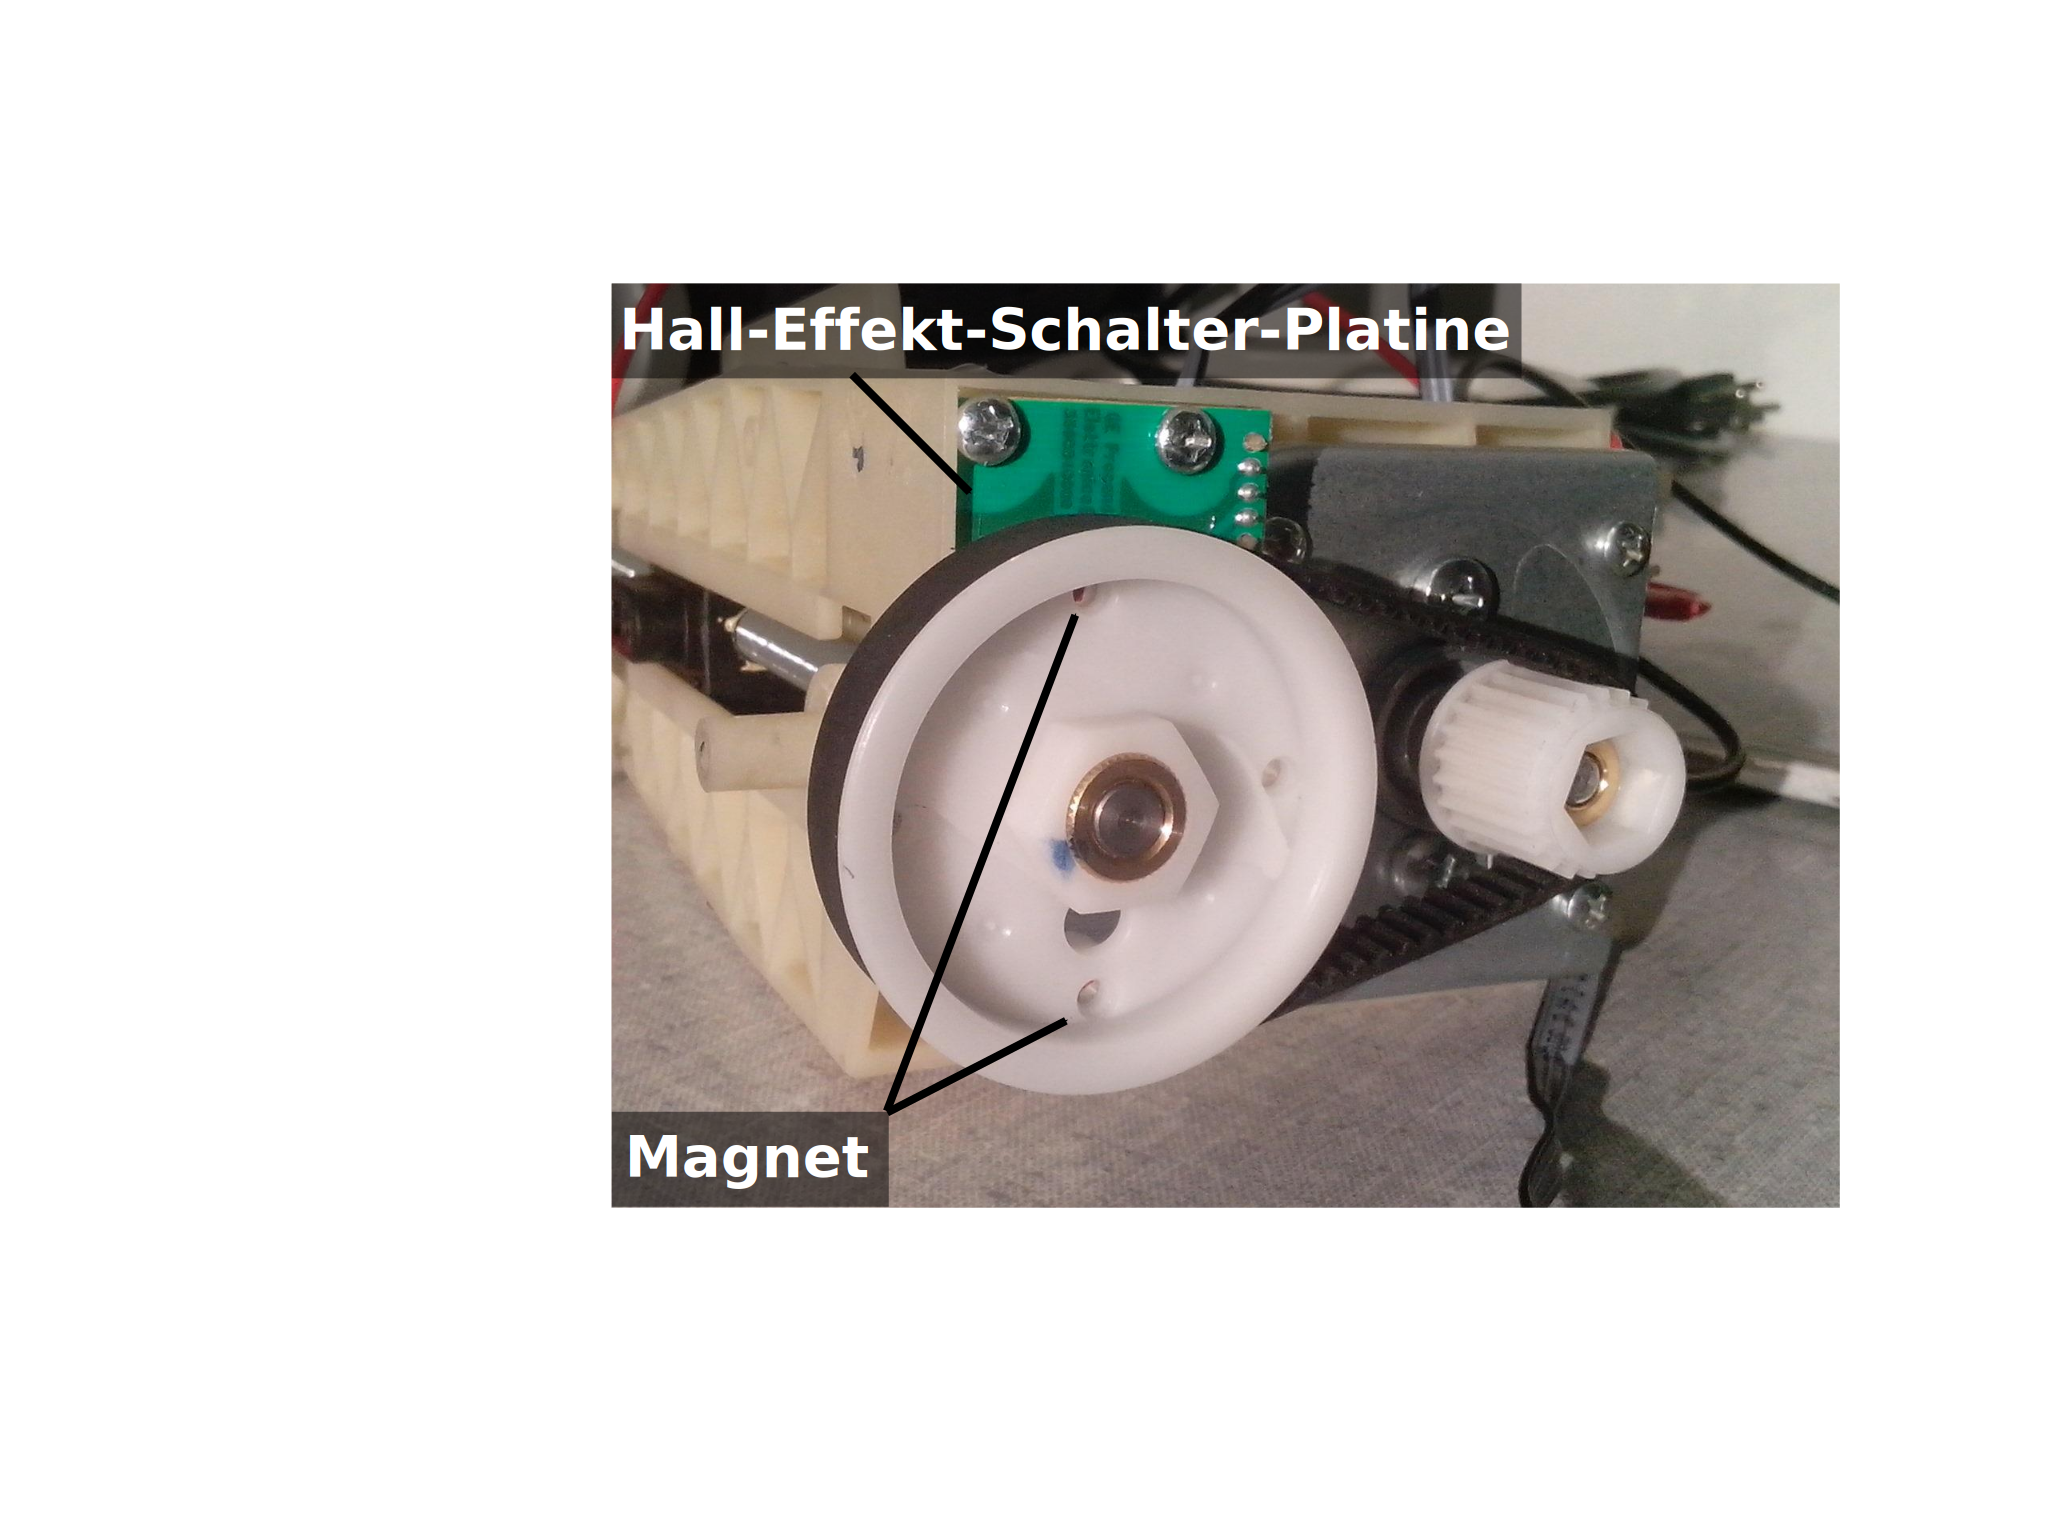
\includegraphics[width=1\textwidth]{../../fig/motor/mech-model-03_01.pdf}
				\caption{Getriebeansicht des Funktionsmusters}
			\end{figure}
		\end{column}
		\begin{column}{0.5\textwidth}
			\begin{block}{Eckdaten}
				\begin{itemize}
					\item Aus Kaffeemaschine
					\item Trapezgewindespindel
					\item Hall-Effekt-Schalter
					\item Universamotor
					\item Ausgeliehen
				\end{itemize}
			\end{block}
		\end{column}
	\end{columns}
\end{frame}

\subsection{Risiken}
\begin{frame}
	\frametitle{Risiken \hfill{} \footnotesize \group}
	\framesubtitle{Risiken \& Massnahmen}
	\begin{block}{Risiken \& Massnahmen}
		\begin{tabular}{l l l}
			Bereich
				& Risiko
				& Massnahme \\
			\hline
			& & \\
			INF	& Kommunikation
				& ??? \\
				& Störeinflüsse bei Bildverarbeitung
				& ??? \\
			& & \\
			ET	& Zeitdruck
				& Terminplan \\
				& ungünstige Annahmen
				& Reserven einplanen \\
			& & \\
			M	& Stabilität, Präzision
				& ??? \\
		\end{tabular}
	\end{block}
\end{frame}
